\documentclass[../main-v1.tex]{subfiles}
\begin{document}
\chapter{Networking \hideme{Mike Kirby and Peter Clarke - in progress}}
\label{ch:netw}

%%%%%%%%%%%%%%%%%%%%%%%%%%%%%%%%
%\section{xyz}
%\label{sec:netw:xyz}  %% fix label accordinean to section


%Kirby - I believe the things in the todo are accomplised. \todo{{\it }Kirby to write first about US side of the network including - US OSG site connectivity, - FNAL connection to \dword{esnet}, Pete then hooks Europe on to this.}

%anne looking at this 3/15

With the DUNE experiment located at two geographically distant sites and having computing resources distributed around the globe, the design and operation of networking will be important to the success of the DUNE experiment. The network requirements can in general be divided between three main areas: %of concern: Far Detector, Near Detector, 
\dword{fd}, \dword{nd} and distributed computing. Assuring that interconnection and bandwidth requirements between each are met with appropriate uptime is necessary for operations and successful physics results. The requirements for each system are based upon current estimates of data rates for both the \dword{fd} and \dword{nd} \dword{daq}, technical networks, and slow control networks.

\section{SURF to Fermilab}

The \dword{fd} networking encompasses the local area network at \dword{surf}, the connection to the wide area network, and the network path back to storage services at \dword{fnal} in Batavia, IL. This network path between the \dword{fd} at \dword{surf} and the \dword{fnal} campus is the most important network path for the DUNE raw data. This path will be used both for transfers of raw data, and also for connectivity between \dword{surf} and operations centers at Fermilab and elsewhere. While operations traffic is expected to use this connection, it should be noted that safety systems will not rely upon the network connection.

The requirements for the network connection between \dword{surf} and \dword{fnal} were explored extensively in the High Energy Physics Network Requirements Review~\cite{bib:osti_1804717} . The primary bandwidth requirement is determined from both the steady-state yearly transfers from the \dword{daq}, and by burst 
%Kirby - it's burst transfers but not just from SNB \fixme{\dword{snb}?}
transfer rates during extended-readout trigger records. The Consortium Interface document between the DUNE \dword{daq} Consortium and the DUNE Computing Consortium and the \dword{daq} specification~\cite{edms:dunedaq} state that no more than 30 Petabytes (PB) of data will be output from the \dword{daq} for permanent storage. This translate into 7.98 Gigabits per second (Gb/s) of steady-state data transfer from \dword{surf} to \dword{fnal}, and includes raw data from beam triggers, cosmic triggers, and calibration runs. 

The most extreme burst requirement considered in the ESNet review was the handling of extended-time trigger records for %SuperNova
\dword{snb} candidates. These trigger records, in contrast to the steady beam and cosmic ray rate,
are expected to occur one to two times/month and involve data volumes of up to 320\,TB/module of uncompressed \dword{fd} data. The ability to produce a reasonably fast pointing signal would be extremely valuable to optical astronomers doing follow-up, especially if the supernova were in a region where dust masks the primary optical signal. The need to be alert to %supernovae 
\dwords{snb} and to quickly transfer and process these data imposes significant requirements on triggering, data transfer, and reconstruction beyond those imposed by the more regular beam-based oscillation physics. For example, an uncompressed \dwords{snb} readout of the first two \dword{fd} modules will be on the order of 320\,TB in size and take a minimum of seven hours to transfer over a 100\,Gb/s network, and then take on the order of 90,000\,CPU-hrs for signal processing at present speeds. If processing takes the same time as transfer, a peak of 10-20,000 cores would be needed. In order to have initial analysis results of a \dwords{snb} trigger record within one day, the network between the  \dword{fd} at \dword{surf} and the \dword{fnal} campus is being designed for a capacity of 100\,Gb/s.  

\hideme{I updated these numbers with the assumption of data not being compressed and the new data volumes from VD} 

As the network will be used for both raw data transfer and for remote operations, there is a requirement to have both a primary and secondary network path between the \dword{fd} and \dword{fnal}. Working in conjuction with ESNet, the Core Computing Division at \dword{fnal} has development a deployment plan for two geographically separate network paths. The map of the proposed paths is shown in Figure~\ref{fig:esnet_network_path_map} with the two paths merging between St. Cloud, MN and the \dword{fnal} campus. The primary path connects network switches at the top of the Ross Shaft (at \dword{surf} in Lead, SD) to \dword{fnal} via ESNet infrastructure. As of February 2022, the primary path is available from Lead, SD 
to \dword{fnal} at limited bandwidth of 10\,Gb/s. In order to complete this path, a vendor will be secured to provide infrastructure between Lead and the Ross Shaft. After completion, the primary path will provide 100\,Gb/s guaranteed bandwidth. The secondary path will provide 10\,Gb/s of network bandwidth and should be available in %CY22 or CY23 
2022 or 2023 and will be from the Yates Shaft (also at \dword{surf}) through Denver, CO to \dword{fnal} via ESNet infrastructure. The networking is expected to be completed in stages with both paths capable of the full design bandwidth by the time that \dword{fd} physics operations commences. A detailed schedule for networking is shown in Figure~\ref{fig:esnet_network_timeline}. Additionally, a tertiary path that utilizes vLAN infrastructure from the South Dakota Higher Education Network (REED) and a southern path through Colorado and Kansas City, KS will provide 10\,Gb/s of bandwidth. During construction, the tertiary path will serve as the primary link to the DUNE \dword{fd} and then revert to a tertiary role once the dedicated primary path is complete.

The network uptime is defined by the capability of the \dword{fd} \dword{daq} system to stage raw data locally in case all connectivity is lost. %The FD
This \dword{daq} is designed to have capacity to store one week of raw data from the detector on local storage at \dword{surf}. %Were connectivity to be lost for an entire week and g
Given the nominal rate of 7.98\,Gb/s from the \dword{daq}, and assuming that the network interface ard (NIC)
%Kirby - fixed locally \fixme{define NIC in glossary pls}
present in the local storage have infinite bandwidth, the additional 92\,Gb/s of bandwidth available on the primary path means that 
were connectivity to be lost for an entire week, 
the backlog in raw data would be cleared within one day of reconnection. And given the presence of three geographically separate paths from \dword{surf} to \dword{fnal}, if all three networks have an uptime of > 90\%, then the expected networking live time (99.9\%) is more performant than the \dword{daq} required live time (98\%) by more than a factor of 10.

\begin{dunefigure}
[ESNet map of network path]
{fig:esnet_network_path_map} 
{A map of the geographically separate primary (blue) and secondary (red) proposed network paths between \dword{surf} and \dword{fnal}. %A map of the geographically separate networking paths proposed for primary (blue) and secondary (red) network paths between \dword{surf} and \dword{fnal}.
}
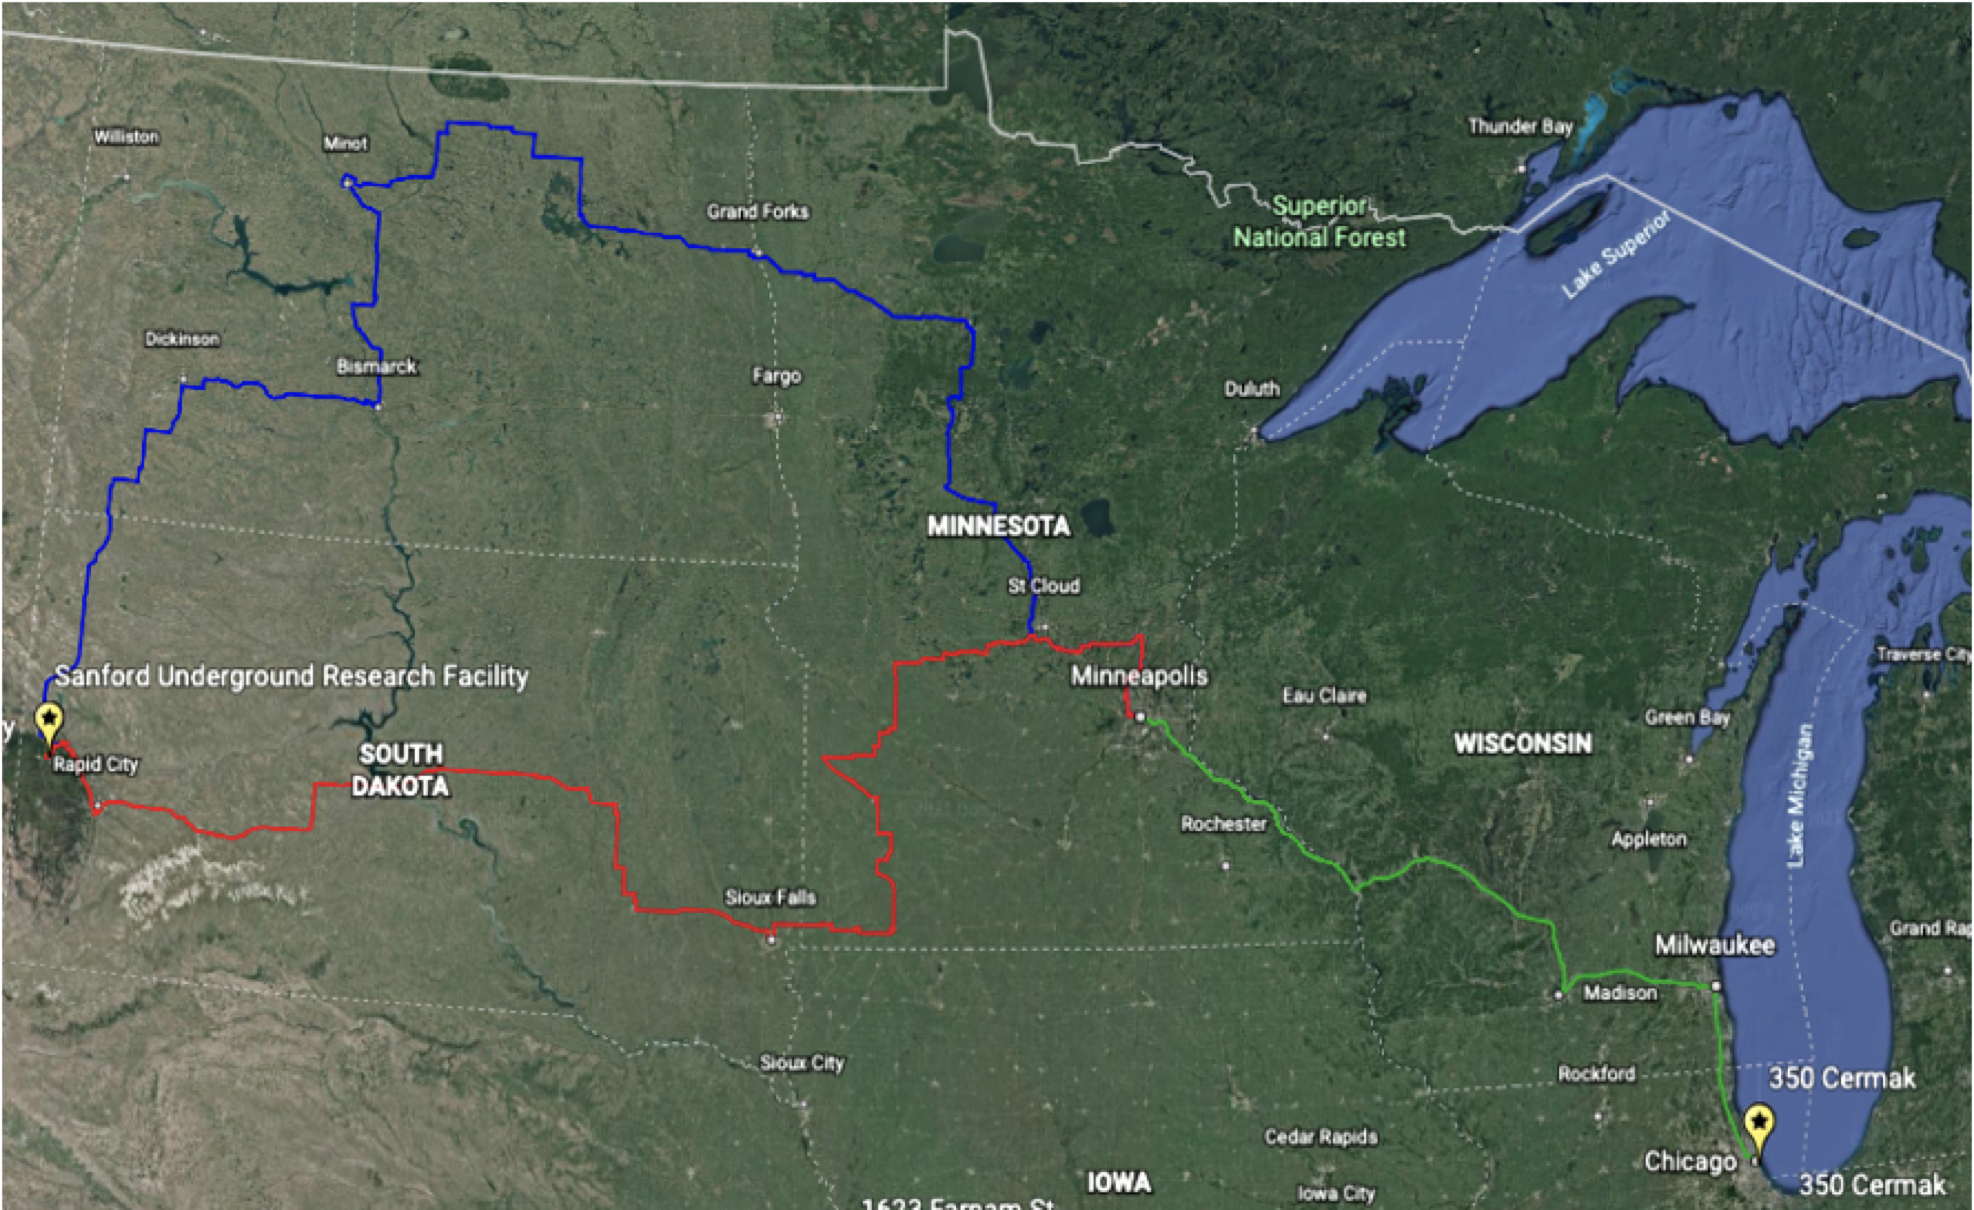
\includegraphics[width=0.9\columnwidth]{graphics/Networking/DUNE_ESNet_network_path.png}
\end{dunefigure}

\begin{dunefigure}
[Networking Timeline]
{fig:esnet_network_timeline} 
{The current timeline for the implementation of networking connection between \dword{surf} and \dword{fnal}.}
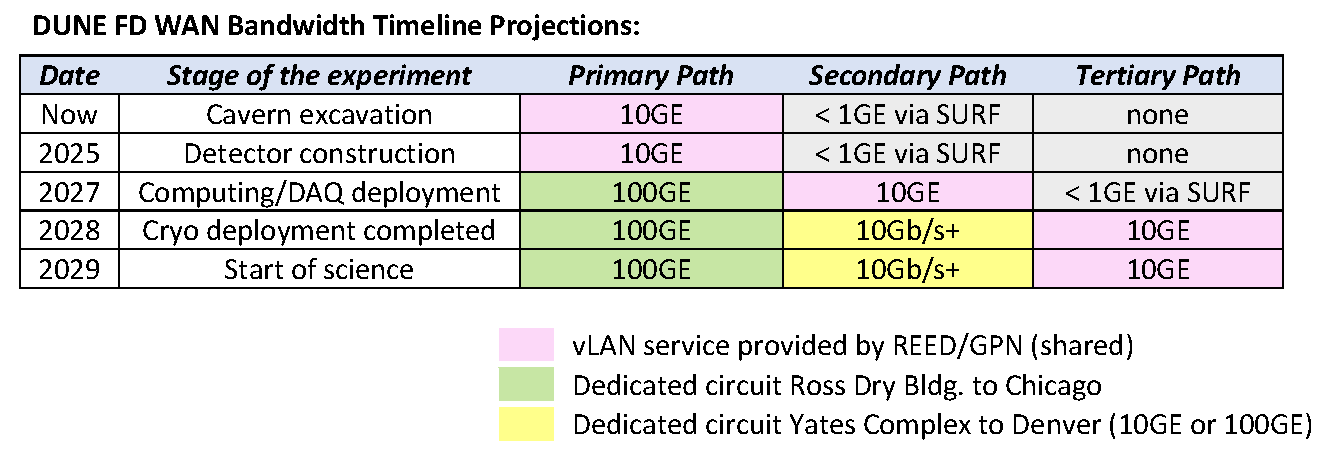
\includegraphics[width=0.9\columnwidth]{graphics/Networking/DUNE_network_Timeline_3-14-2022.png}
\end{dunefigure}


\section{Far and Near Site Local Area Networks}

The local area network (LAN) for the Far and Near Sites will be designed, installed, and commissioned as a collaboration between the \dword{dune} \dword{daq} %Group 
consortium and the \dword{fnal} Core Computing Division (CCD). The \dword{daq} has provided requirements to CCD and preliminary designs of the LAN have begun. The installation of networking infrastructure at \dword{surf} will be paid for by the %\dword{dune} 
\dword{usproj} Project 
%Kirby - I believe that DAQ is on project and have spoken with the DAQ group who has said they are paying for the networking hardware and installation. \fixme{is that right? or paid for by int'l DUNE?}
and is scheduled to start in %FY26. 
2026. Once network installation has begun, there is a joint responsibility between \dword{surf} and CCD network experts to configure and maintain the interface with external high-capacity networking for data transfers to storage at \dword{fnal}. The installation of LAN at the Near Site is planned to begin in %FY29
2029, , and follows a similar set of responsibilities as at \dword{surf}. The \dword{daq} group will provide requirements and CCD providing design, commissioning, and operational support for the Near Site LAN.

%\todo{Some of this may move into cooperation section}
\section{Global Connectivity}
Connection to European sites is accomplished via the Energy Sciences network (\dword{esnet}),
the pan-European research network (\dword{geantnet}) and \dword{nren}.
The current aggregate  transatlantic bandwidth is of the order of a Tbit/s, of which 400\,Gbit/s is from  \dword{esnet} (Boston, New York and Washington DC)
to \dword{geantnet} (London, Amsterdam and Geneva (\dword{cern})).
\dword{geantnet} in turn peers with the \dword{nren}   in each participating country, where details
pertaining to each DUNE site vary. As an example, in the UK the
\dword{nren} is JISC-JANET, which at the time of writing has a 400\,Gbit/s core and connects to the GridPP-RAL site redundantly at 100\,Gbits/s.
Similarly the CC-IN2P3 site in France is connected to RENATER at 100\,Gbits/s, and the FZU site in the Czech Republic is connected to CESNET
at 100\,Gbit/s Gbit/s.  DUNE expects all participating countries to
ensure that as part of their pledges of CPU and storage capacity, %that
their sites %offered 
have commensurate network connections. %We do not expect any 
No systematic issues are expected to arise, and none have done so in the
WLCG/LHC context. DUNE participates in the worldwide \dword{hep} Network
coordination body which meets twice per year  (the LHCOPN/LHCONE Group).



 Layer-3\footnote{https://en.wikipedia.org/wiki/Network\_layer} \dword{vrf} provision is now very prevalent in \dword{hep}. 
%Kirby - included link to wiki article. \fixme{what does layer-3 mean?}
 \dwords{vrf} provide a logical routing overlay that can allow for traffic engineering to utilize high-capacity paths where needed. The \dword{lhc} community uses a \dword{vrf} called LHCONE, and this has also been used for DUNE traffic along with other non-\dword{lhc} experiments such as Belle II. 
At present DUNE is agnostic %to 
regarding the use of LHCONE, and since \dword{fnal} is connected to LHCONE it can easily accommodate sites with or without such provision.
Investigations are currently underway to determine the technical requirements for the creation of a separate DUNEONE \dword{vrf} were it to ever be required. It is, however, not currently foreseen, and does not form part of our baseline planning.
\end{document}